% Appendix A

\chapter{Trajectories} % Main appendix title

\label{AppendixA} % For referencing this appendix elsewhere, use \ref{AppendixA}

\section{Figures of the Trajectories used in the Experiments}

\begin{figure}[th]
\centering
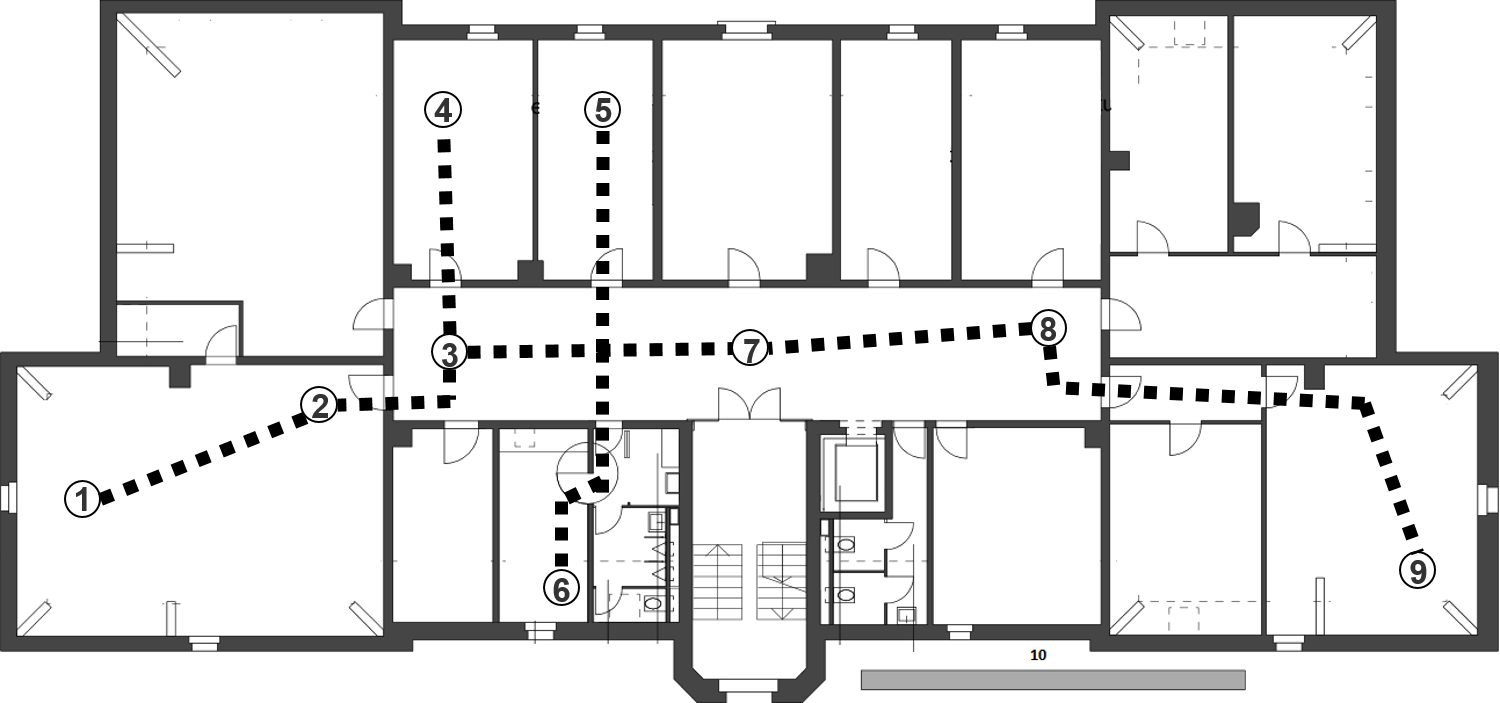
\includegraphics[width=1.0\textwidth]{Figures/trajectory1}
\decoRule
\caption[Trajectory 1]{Checkpoints and path of trajectory 1.}
\label{fig:trajectory1Appendix}
\end{figure}

\begin{figure}[th]
\centering
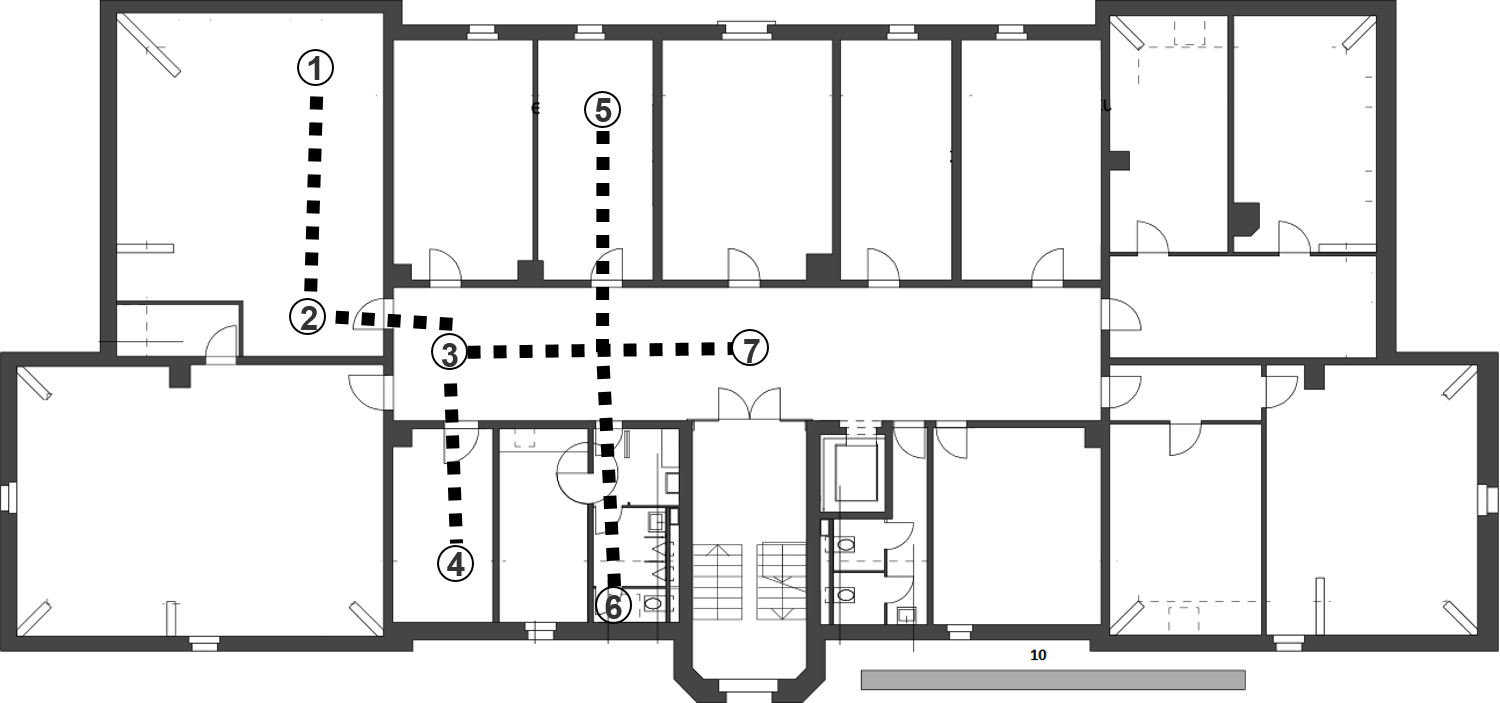
\includegraphics[width=1.0\textwidth]{Figures/trajectory2}
\decoRule
\caption[Trajectory 2]{Checkpoints and path of trajectory 2.}
\label{fig:trajectory2}
\end{figure}


\begin{figure}[th]
\centering
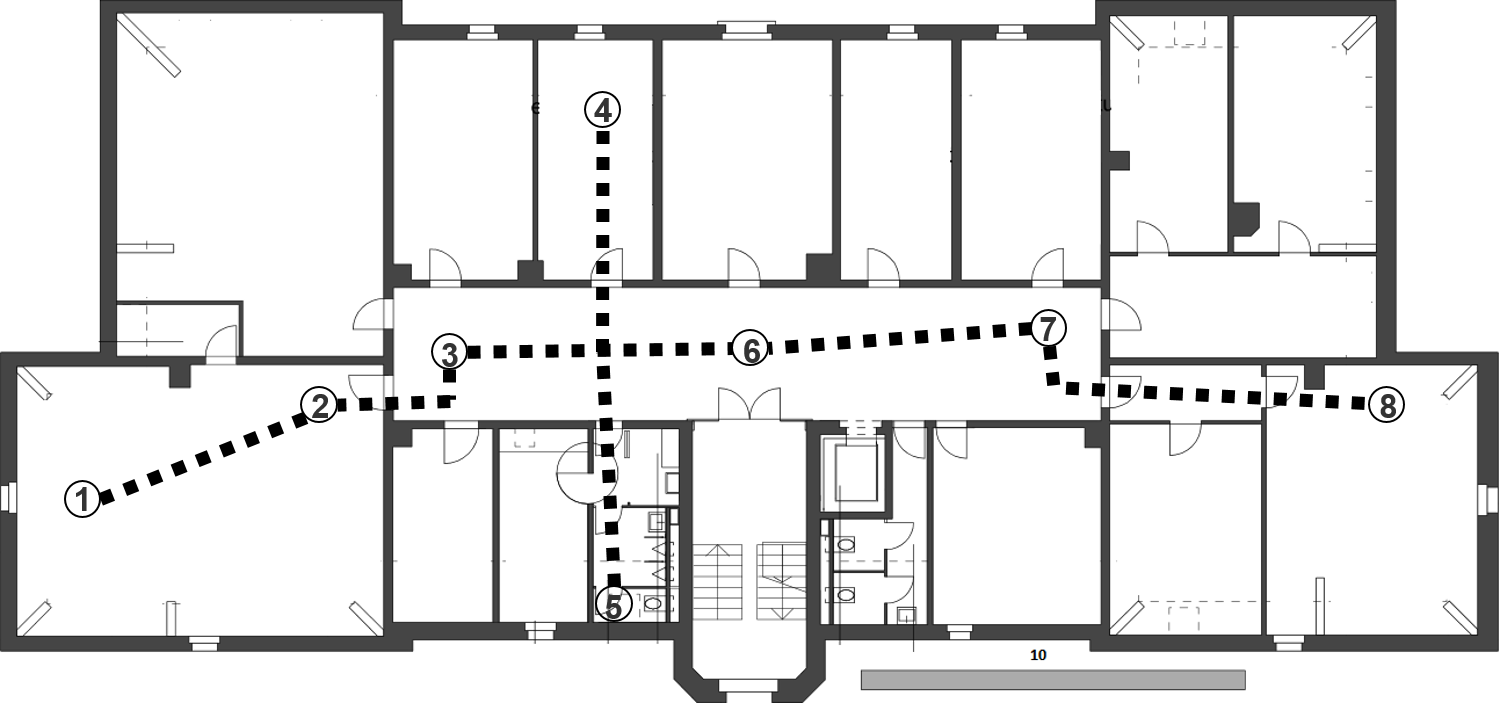
\includegraphics[width=1.0\textwidth]{Figures/trajectory3}
\decoRule
\caption[Trajectory 3]{Checkpoints and path of trajectory 3.}
\label{fig:trajectory3}
\end{figure}


\begin{figure}[th]
\centering
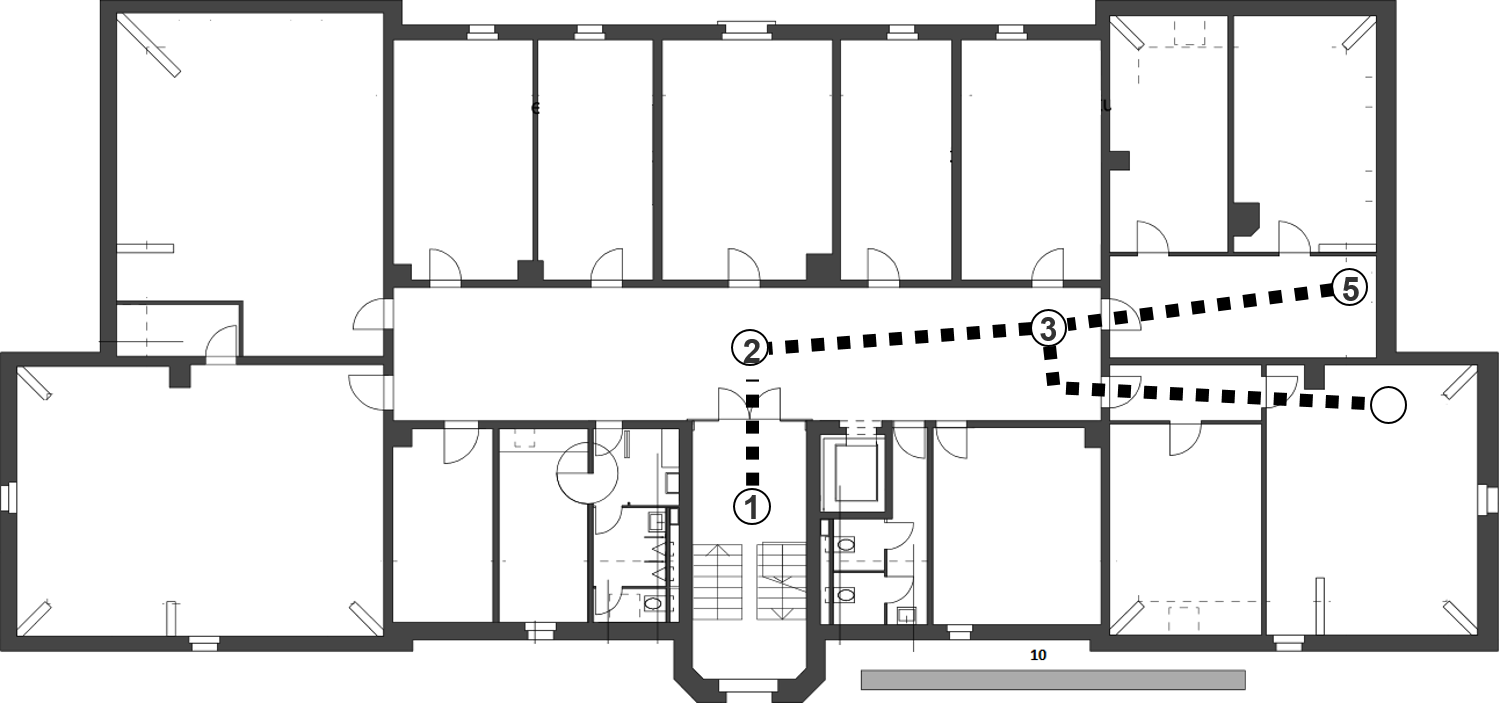
\includegraphics[width=1.0\textwidth]{Figures/trajectory4}
\decoRule
\caption[Trajectory 4]{Checkpoints and path of trajectory 4.}
\label{fig:trajectory4}
\end{figure}

\begin{figure}[th]
\centering
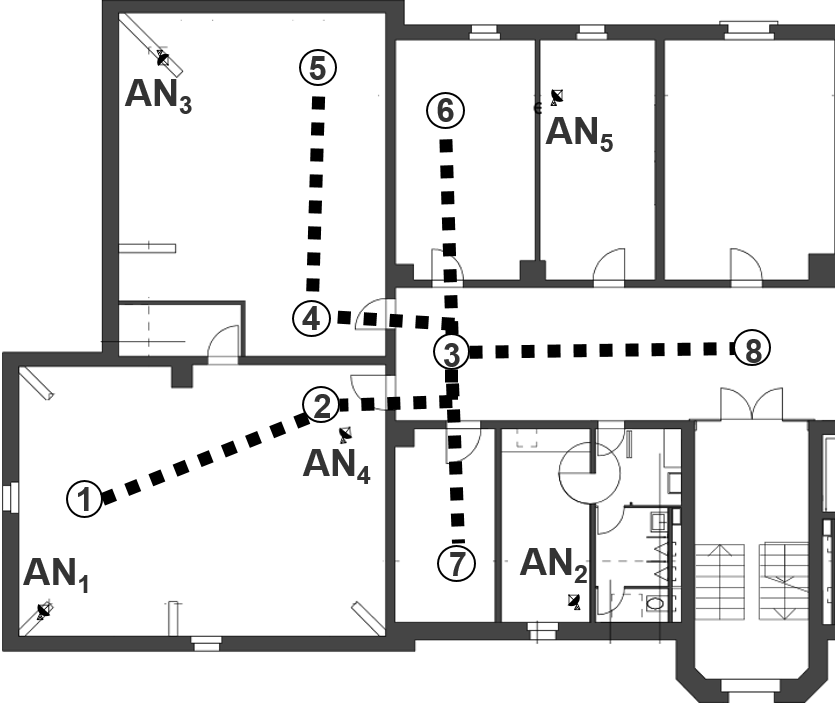
\includegraphics[width=1.0\textwidth]{Figures/trajectory5_withAnchors}
\decoRule
\caption[Trajectory 5]{Checkpoints and path of trajectory 5 with anchor positions.}
\label{fig:trajectory5_withAnchorsAppendix}
\end{figure}
